\documentclass[11pt, a4paper]{article}

\usepackage[utf8]{inputenc}
\usepackage[french]{babel}
\usepackage[T1]{fontenc}
\usepackage{verbatim}
\usepackage{color}
\usepackage{listings}
\usepackage{graphicx}

% $1 : fichier source
% $2 : langage
\newcommand{\addCode}[2]{%

  % Configuration de la coloration syntaxique du code
  \definecolor{colKeys}{rgb}{0,0,1}
  \definecolor{colIdentifier}{rgb}{0,0,0}
  \definecolor{colComments}{rgb}{0,0.5,1}
  \definecolor{colString}{rgb}{0.6,0.1,0.1}

  % Configuration des options 
  \lstset{%
    language = #2,%
    identifierstyle=\color{colIdentifier},%
    basicstyle=\ttfamily\scriptsize, %
    keywordstyle=\color{colKeys},%
    stringstyle=\color{colString},%
    commentstyle=\color{colComments},%
    columns = flexible,%
    %tabsize = 8,%
    showspaces = false,%
    numbers = left, numberstyle=\tiny,%
    frame = single,frameround=tttt,%
    breaklines = true, breakautoindent = true,%
    captionpos = b,%
    xrightmargin=10mm, xleftmargin = 15mm, framexleftmargin = 7mm,%
  }%
    \begin{center}
    \lstinputlisting{#1}
    \end{center}
}

\title{Spécification des fonctions d'un pilote de périphérique de type capteur}
\author{Paul \textsc{Adenot} \and \'{E}tienne \textsc{Brodu}}
\date{}

\setlength{\parindent}{0cm}

\begin{document}
\maketitle

\newcommand{\kw}[1]{\texttt{#1}}

\newcommand{\DescFonction}[4]{%
	\texttt{\Huge{#1}} \\ 
	\raisebox{0.5em}{\rule{\textwidth}{0.1ex}}\\
	\textbf{\large{Synopsis}} \\
	\texttt{#2} \\
	\textbf{\large{Description}} \\
	#3 \\
	\textbf{\large{Valeur de retour}} \\
	#4 
	\vspace{1cm}
}

\section{Documentation de l'API}
\DescFonction{open}
{int open(const char* filename, int flags, int perms)}
{Ouvre le capteur désigné par \kw{filename}, et renvoie une descripteur de fichier (\emph{file descriptor}), qui l'identifie au sein du programme. \kw{flags} indique le mode d'ouverture, et doit être fixé à \kw{O\_RDONLY}, les capteurs étants en lecture seule. Plusieurs capteurs peuvent être ouvert au sein du même programme. Si un même capteur est ouvert plusieurs fois au sein du même programme, alors plusieurs descripteurs de fichiers seront disponible pour lire sur un même capteur. Si le fichier précisé dans le premier paramêtre (\kw{filename}) n'existe pas, l'appel échoue, et \kw{open} retourne immédiatement, avec la valeur -1.}
{Si l'appel reussi, un descripteur de fichier (entier positif). Sinon, -1.}

\DescFonction{creat}
{int creat(const char *pathname, int mode);}
{Le comportement de cette fonction est similaire à celui de la fonction \kw{open}}
{Les valeurs de retours sont les mêmes que celles de la fonction \kw{open}.}

\DescFonction{close}
{int close(int fd);}
{Ferme le capteur désigné par le descripteur de fichier \kw{fd}. Celui-ci ne sera plus utilisable dans le programme.
Si le paramêtre \kw{fd} est invalide (i.e. négatif ou ne correspondant pas à un descripteur de fichier valide), \kw{close} retourne -1.}
{Si l'appel réussi, 0 est renvoyé, -1 sinon.}

\DescFonction{remove}
{int remove(const char *pathname);}
{Ferme le capteur désigné par \kw{pathname}. Il ne sera plus utilisable au sein du programme.
Si \kw{pathname} est invalide (le fichier n'existe pas, ou n'est pas ouvert au sein du programme), alors l'appel échoue.}
{SI l'appel réussi, 0, -1 sinon.}

\DescFonction{read}
{int read (int fd, char *buffer, size\_t maxbytes);}
{Lit un message d'un capteur désigné par \kw{fd}, et le place dans l'adresse pointé par \kw{buffer}.
Si un message est disponible, alors il est placé dans à l'adresse \kw{buffer}, mais n'est pas \emph{consommé}. Plusieurs appels successifs à \kw{read} sur un même file descriptor peuvent donc donner le même message.
Un message lu sur un capteur est du type \kw{capt\_msg}, qui est défini de la manière suivante :
\addCode{ressources/code.c}{c}~}
{Si aucun message n'est disponible (par exemple dès la mise sous tension du capteur, et en attente de ma première information), -1 est renvoyé, sinon, un entier positif, correspondant à la taille lue (\kw{TAILLE\_MSG}) est renvoyée.}

\DescFonction{write}
{int write (int fd, char *buffer, size\_t maxbytes);}
{Appel non supporté, les capteurs sont en lecture seule. Pour faire une opération sur un capteur, utiliser \kw{ioctl}.}
{N.A.}
	
\DescFonction{ioctl}
{int ioctl(int fd, int request, int value);}
{Configuration du pilote.
Si \kw{request} est inférieur ou égal à 255, ioctl comprend qu'il s'agit du numero du périhpérique à remplacer.
L'adresse du nouveau périphérique branché doit être passé en \kw{value}. Cette partie sera spécifiée ultérieurement.
Les valeurs de \kw{request} plus élevées sont réservées, et pourront correspondre à d'autres fonctionnalités, dans le futur.}
{0 en cas de succès, -1 sinon.}

\section{Structure des données}

\subsection{table\_capteur}
Ce tableau contient 15 pointeurs vers des structures decrivant chaque capteur.
L'index du tableau servant d'identifiant logique au sein du driver.
Structure décrivant un capteur :
\addCode{ressources/descr_capt.c}{c}

\subsection{table\_buffer}
Ce tableau contient 15 pointeurs vers le dernier message du capteur dont l'index du tableau est l'identifiant logique.

\section{Conception graphique}

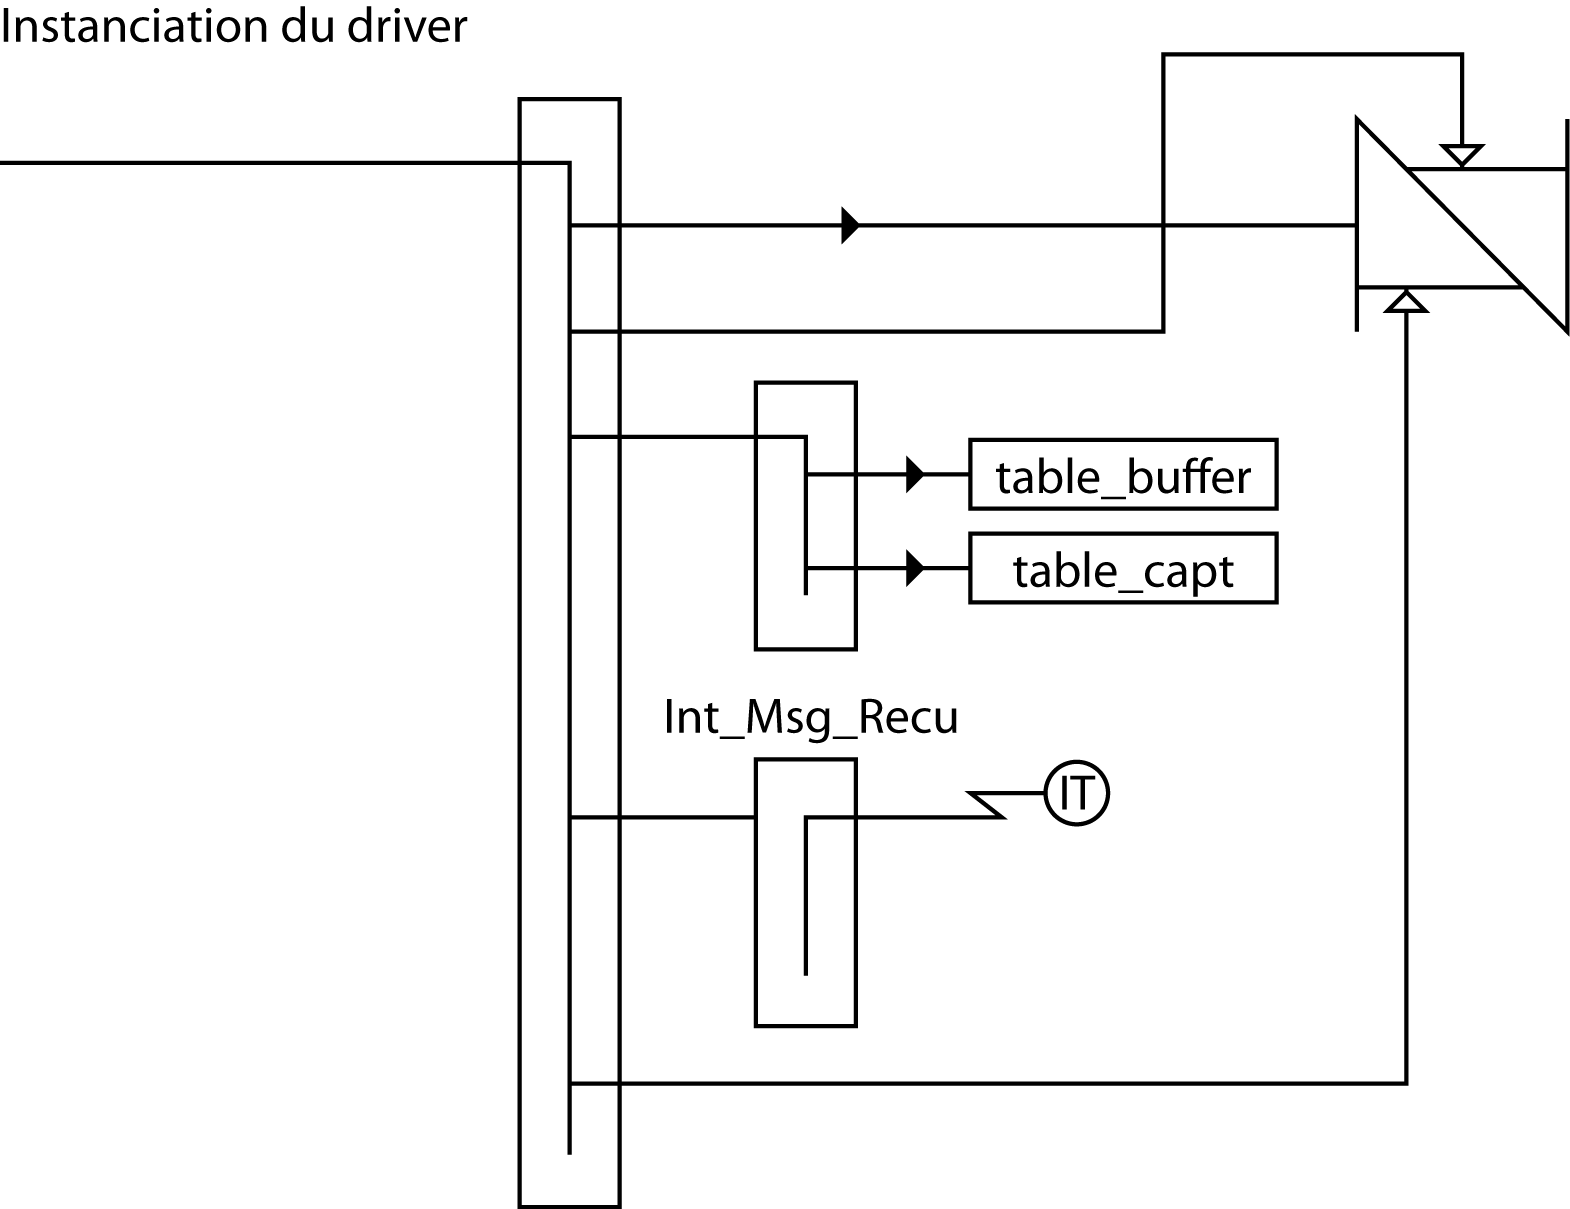
\includegraphics{ressources/init.png}\\~\\
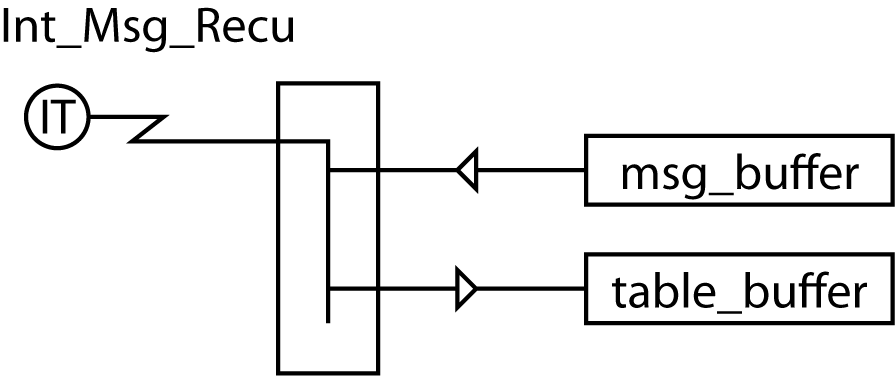
\includegraphics{ressources/int.png}\\~\\
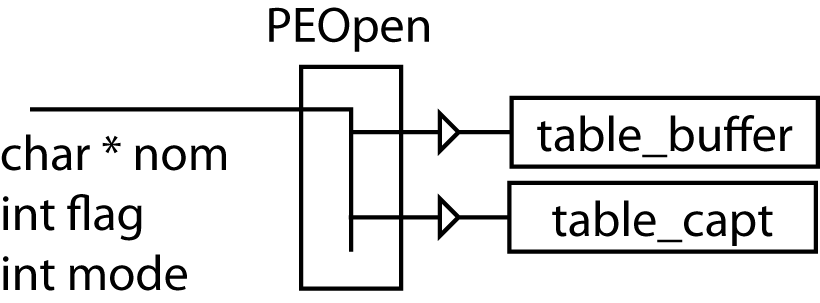
\includegraphics{ressources/open.png}\\~\\
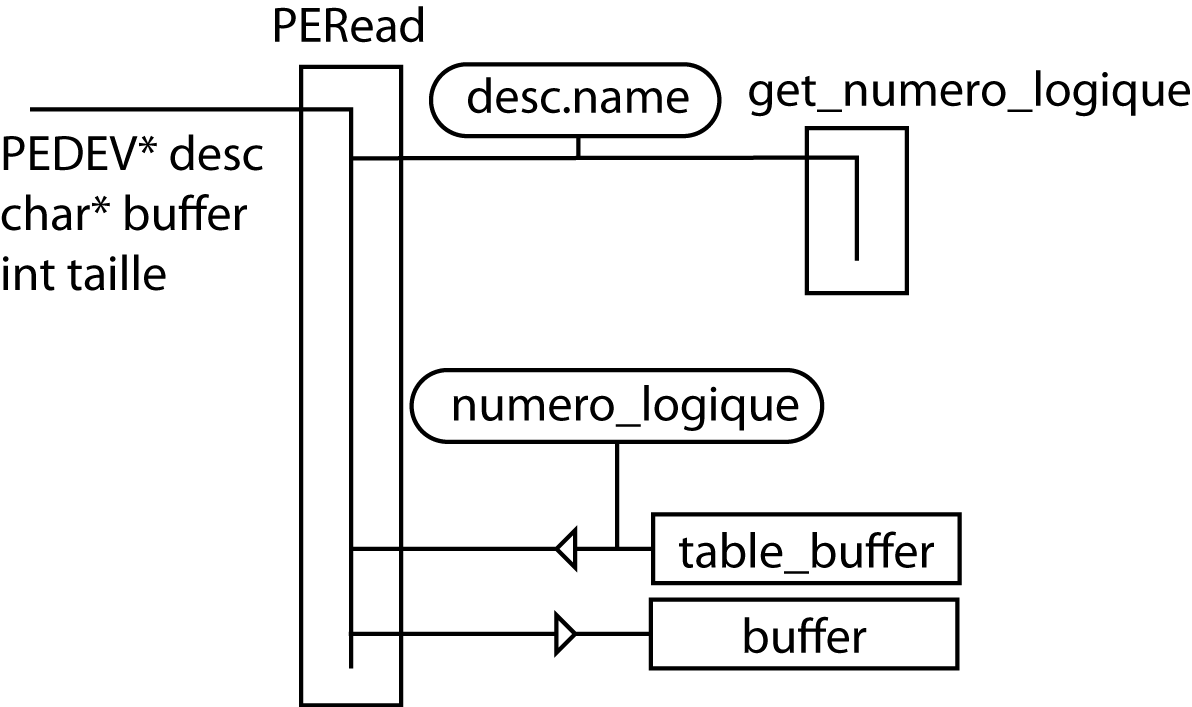
\includegraphics{ressources/read.png}\\~\\
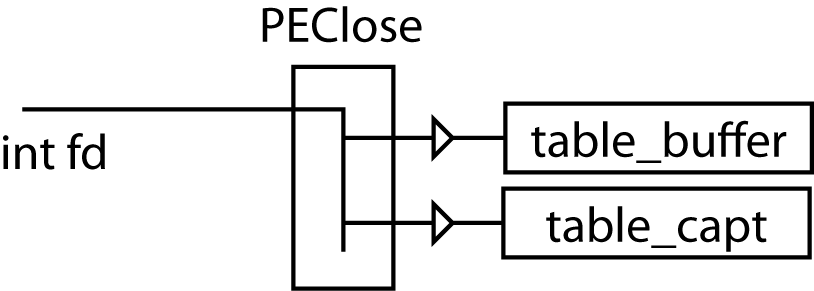
\includegraphics{ressources/close.png}

\end{document}


